\documentclass[12pt]{article}
\usepackage{amssymb,amsmath}
\usepackage{graphicx}
\usepackage{textcomp}
\usepackage{listings}
\usepackage{color}
\usepackage{courier}
\usepackage{url}
\usepackage{changepage}
\usepackage{enumitem}
\newcommand{\code}[1]{\texttt{#1}}
\newcommand{\home}{{\raise.17ex\hbox{$\scriptstyle\mathtt{\sim}$}}}
%\usepackage{geometry}
%\geometry{top=1.0in, bottom=1.0in, left=1.5in, right=1.0in}


\begin{document}
\pagenumbering{gobble}
\begin{center}
  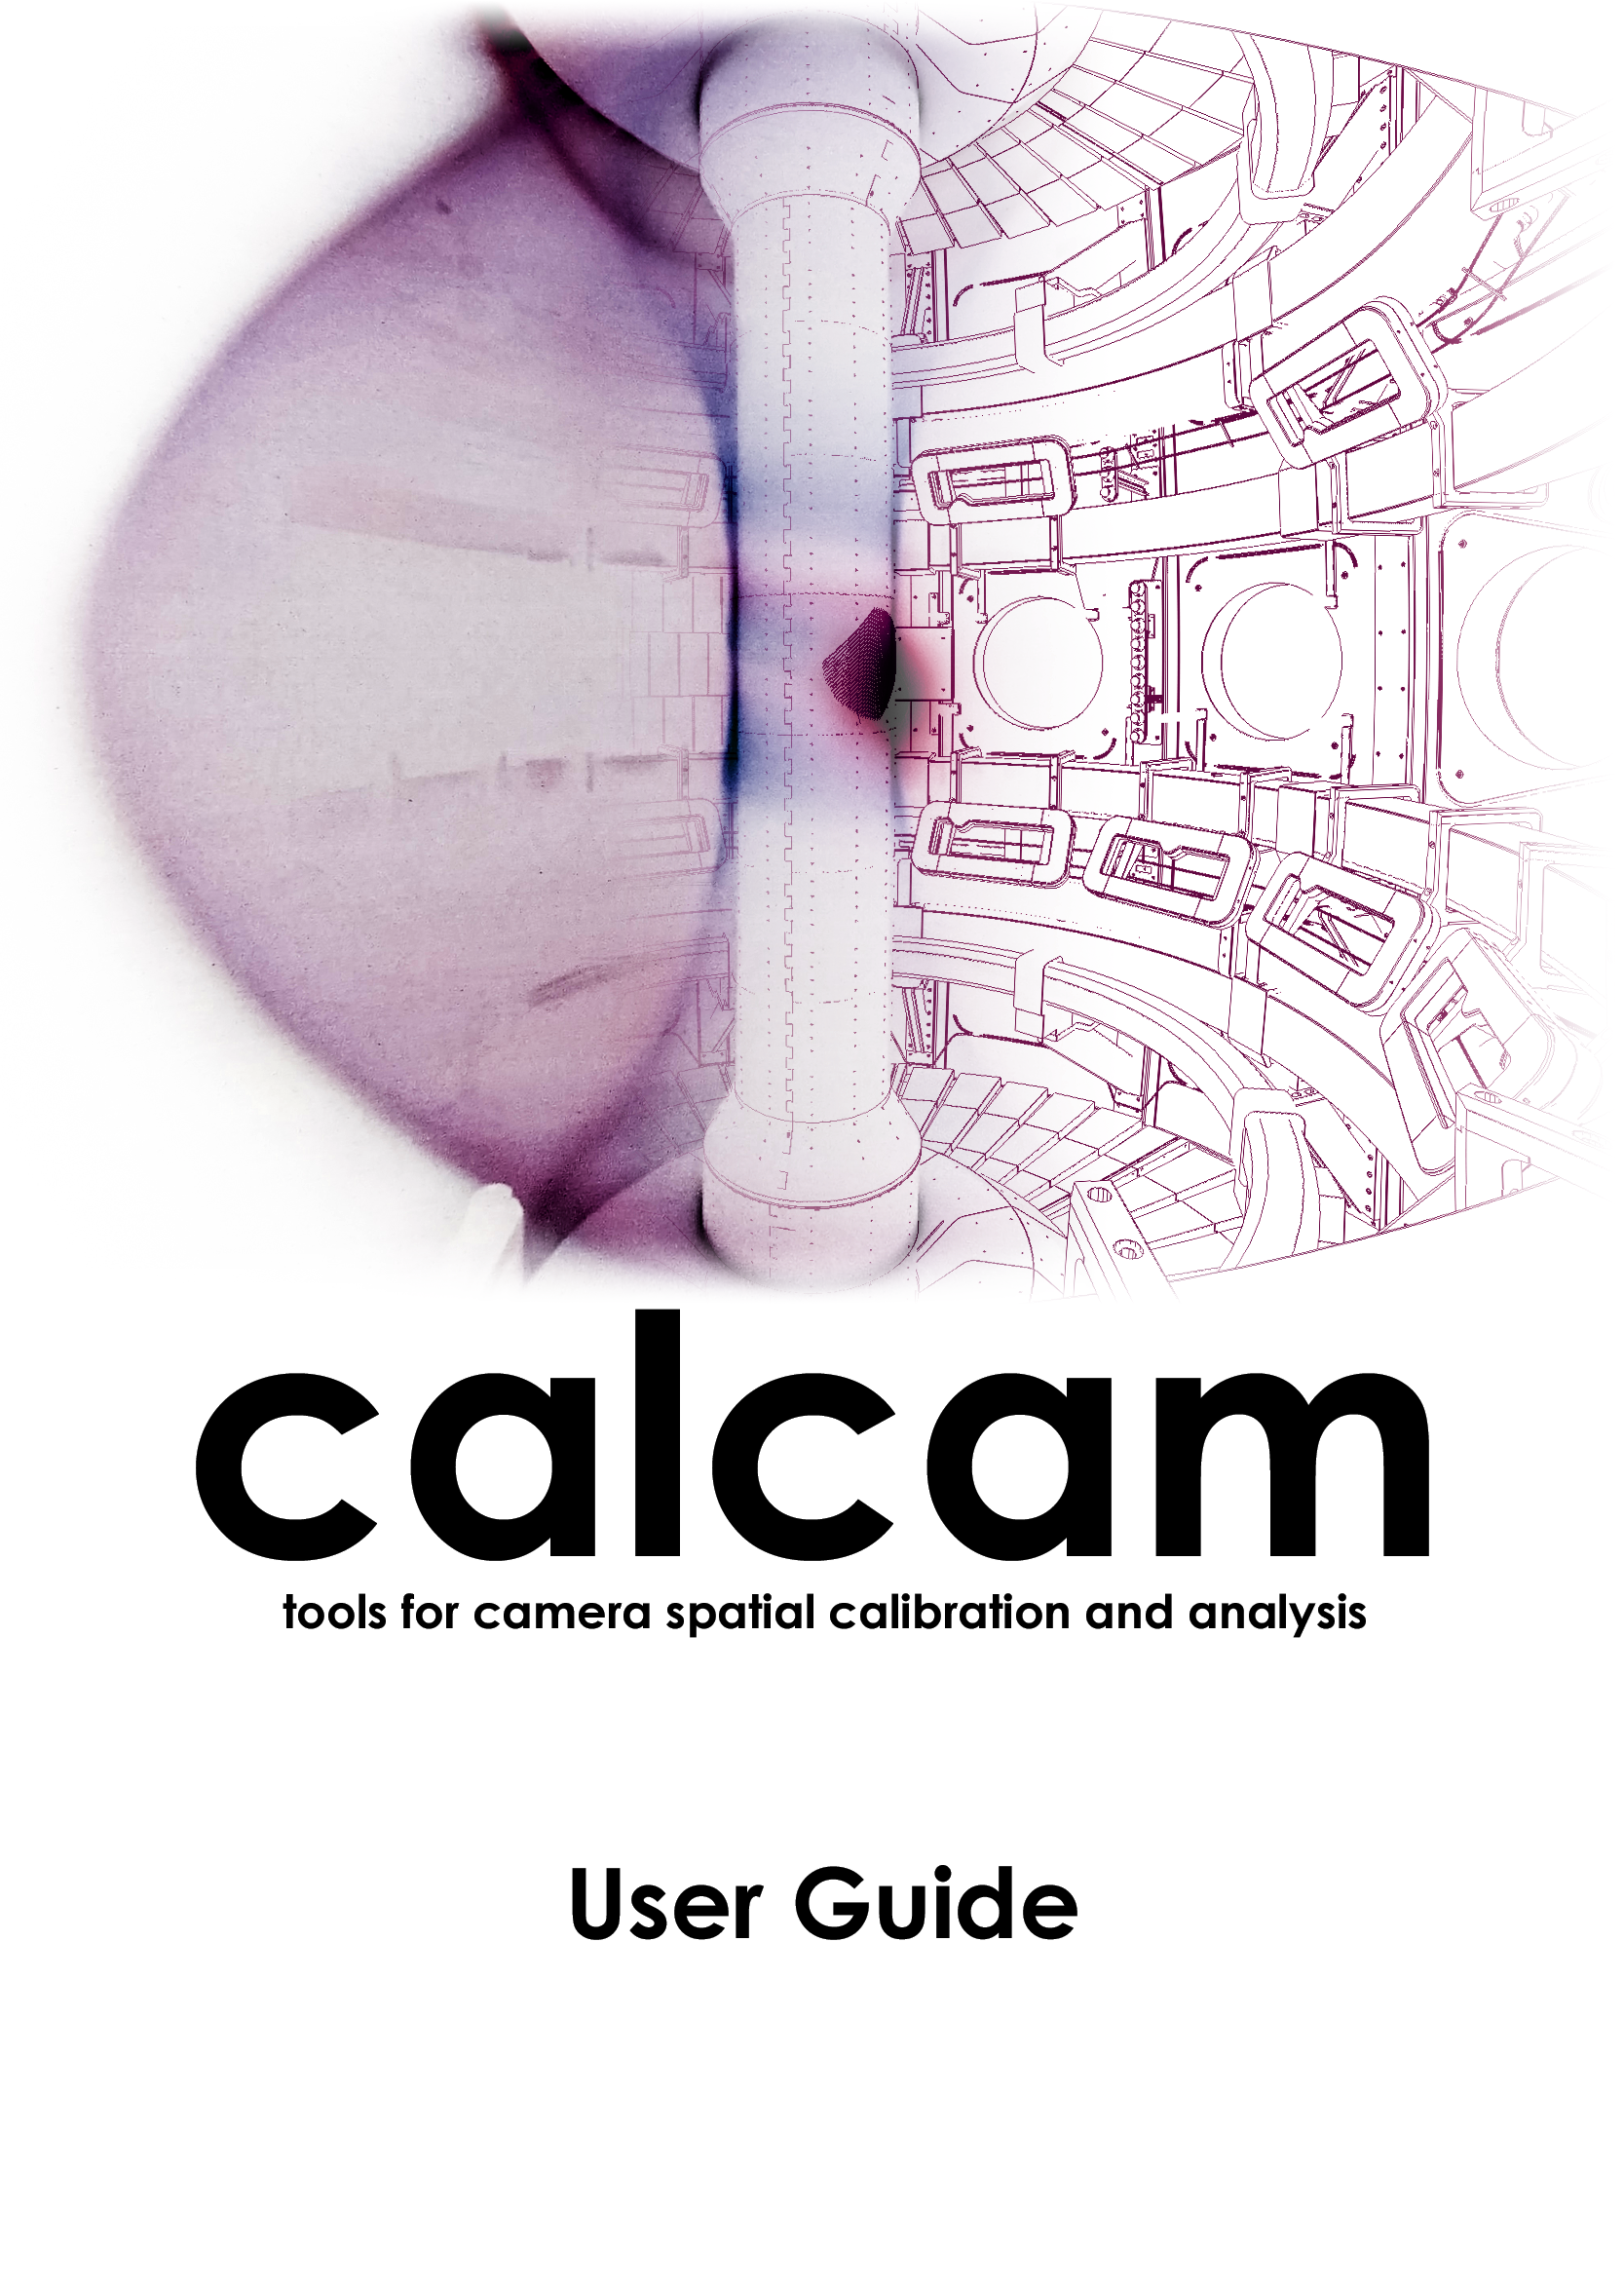
\includegraphics[width=\textwidth]{coverpage.png}
\end{center}


\newpage
\tableofcontents
\newpage
\pagenumbering{arabic}


\section{Introduction \& Background}

\subsection{Purpose \& Scope of Calcam}

Calcam is a python package whose purpose is to provide tools to spatially calibrate camera diagnostic syetems, i.e. to calibrate the mapping between pixel coordinates in camera data and 3D coordinates in real space in the lab. Calibrations are based on matching known features in camera images and features on a CAD model of the scene being observed. Calcam provides a graphical user interface for performing the calibration, and a Python API which provides tools to use these calibrations as part of your data analysis process.


\subsection{Camera View Models}
Calcam works by fitting a model which describes the relationship between 3D real-world coordinates and image coordinates. It supports two different models: one for ``conventional'' perspective projection lenses and one for ``fisheye'' projection lenses. In both cases, we wish to relate the coordinates of a point $(X,Y,Z)$ in the lab frame to its pixel coordinates $(x{_p},y{_p})$ in the camera image. First, we must consider the position and viewing direction of the camera in the lab frame, which is described by a 3D translation and rotation. The translation and rotation parameters are known as the {\it extrinsic} parameters in the model.  Knowing these, we can apply a suitable translation and rotation to obtain the point of interest's coordinates in the {\it camera frame}: a 3D real space coordinate system where the camera pupil is at the origin and the camera looks along the positive $Z$ axis. We denote the coordinates of our point of interest in the camera frame as $(X^\prime,Y^\prime,Z^\prime)$. 

In order to find the pixel coordinates of this point in the camera image, we start with a simple perspective projection, where the height of an object in the image is inversely proportional to its distance from the camera pupil:

\begin{equation}
\begin{pmatrix}x_n\\y_n\end{pmatrix} = \begin{pmatrix}X^\prime/Z^\prime\\Y^\prime/Z^\prime\end{pmatrix}.
\label{eqn:cmmodel_pinhole}
\end{equation}

\noindent The ``normalised'' coordinates $(x_n,y_n)$ are then transformed by a model which describes the image distortion due to the optical system. This model depends on the lens projection being assumed, and models for the perspective and fisheye lens types are described in the following sections. Here we simply denote the resulting distorted normalised coordinates as $(x_d, y_d)$. Finally, the normalised, distorted coordinates are related to the actual pixel coordinates $x_p, y_p$ in the image plane by multiplication with the ``camera matrix'':

\begin{equation}
\begin{pmatrix}x_p\\y_p\\1\end{pmatrix} = \begin{pmatrix}f_x & 0 & c_x \\ 0 & f_y & c_y\\0 & 0 & 1\end{pmatrix}\begin{pmatrix}x_d\\y_d\\1\end{pmatrix}.
\label{eqn:cammatrix}
\end{equation}

\noindent Here $f_x$ and $f_y$ are the effective focal length of the imaging system measured in units of detector pixels in the horizontal and vertical directions, and are  expected to be equal for square pixels and non-anamorphic optics. $c_x$ and $c_y$ are the pixel coordinates of the centre of the perspective projection on the sensor, expected to be close to the detector centre. The parameters in the camera matrix, along with those describing the distortion model, constitute the {\it intrinsic} camera parameters, i.e. they are characteristic of the camera and optical system and are independent of how that system is placed in the lab.

\subsubsection{Perspective Lens Distortion Model}

The image distortion model for perspective projection lenses takes in to account radial (barrel or pincushion) distortion, and tangential (wedge-prism like, usually due to de-centring of optical components) distortions. The equation relating the undistorted and distorted normalised image coordinates in this model is:

\begin{equation}
\begin{pmatrix}x_d\\y_d\end{pmatrix} = \left[ 1 + k_1r^2 + k_2r^4 + k_3r^6\right]\begin{pmatrix}x_n\\y_n\end{pmatrix} +  \begin{pmatrix}2p_1x_ny_n + p_2(r^2 + 2x_n^2)\\p_1(r^2 + 2y^2) + 2p_2x{_n}y{_n}\end{pmatrix},
\label{eqn:perspective_distortion}
\end{equation}

\noindent where $r = \sqrt{x_n^2 + y_n^2}$, and $k_n$ and $p_n$ are radial and tangential distortion coefficients, respectively. The polynomial in $r^2$ in the first term describes the radial distortion while the second term represents tangential distortion.

\subsubsection{Fisheye Lens Distortion}

The fisheye distortion model only includes radial fisheye distortion. Unlike the perspective projection model, the polynomial describing the radial distortion is a function of an anglular distance from the centre of perspective, rather than a linear distance in the image:

\begin{equation}
\begin{pmatrix}x_d\\y_d\end{pmatrix} = \frac{\theta}{r}\left[ 1 + k_1\theta^2 + k_2\theta^4 + k_3\theta^6 + k_4\theta^8\right]\begin{pmatrix}x_n\\y_n\end{pmatrix},
\label{eqn:fisheye_distortion}
\end{equation}

\noindent where $r = \sqrt{x_n^2 + y_n^2}$ and $\theta = \tan^{-1}(r)$.


\subsection{Image Coordimate Conventions}
Calcam follows the convention of using matrix/linear algebra style pixel coordinates for images, which is consistent with the way images are stored and addressed in 2D arrays. In this convention, the origin $(0,0)$ is in the centre of the pixel in the top left corner of the image. The $y$ axis runs from top to bottom down the image and the $x$ axis runs horizontally left to right. It is important to note that since 2D arrays are indexed \code{[row, column]}, arrays containing images are indexed as \code{[y,x]}. However, functions which deal with image coordinates are called as \code{function(x,y)}. This is consistent with the way image coordinates are delt with in OpenCV.

\subsubsection{Original and Display Coordinates}
\label{sec:im_coords}
In camera diagnostics, the data comes out of the camera with some intrinsic orientation which may not be the `right way up' in terms of easily looking at or understanding the images, e.g. if the camera is mounted upside down or the image is flipped by a mirror on the optical path. It is therefore desirable to work with the image transformed to be the `right way round'. However, when performing bulk, programmatic analysis of video data it is not necessary or advantageous to perform this transformation, and is more efficient to work with the raw data as it comes out of the camera or is stored. Calcam therefore uses the concept of `Display' and `Original' image coordinates (thanks to Valentina Huber for this idea, and coining the phrase). Consider an object at a specific point in an image. Its coordinates in the camera image, as read straight from the camera, are the `original' coordinates. If the image is transformed to be the `right way up', the object's coordinates in the image will now be different. These coordinates in the `right way up' image are called `Display' coordinates. Calcam keeps track of the transofmration between original and display coordinates, so that the results can be used with raw data as it comes from the camera as well as processed `right way up' data. It is therefore highly recommended that you do not perform any geometrical transformations to images before loading them in to calcam for calibration, but make all these adjustments within calcam. This will leave the option open for using the raw data more efficiently in your analysis.

By default, calcam functions work with display coordinates unless specified otherwise. This is because the underlying openCV camera model fitting requires that the image being calibrated is not flipped, horizontally or vertically (this would add a minus sign to the pinhole projection which is not supported by the code). This is also an important point when calibrating images: ensure the image is not horizontally or vertically flipped when performing calibrations!

\subsection{About this User Guide}
This is the initial, somewhat rough and incomplete version of the Calcam user guide, written by Scott Silburn (\url{scott.silburn@ukaea.uk}). Feedback on both the code and the user guide are welcome. The installation and setup and API documentation sections assume a reasonable familiarity with the Python language.


\section{Getting Started \& Configuration}

\subsection{Hardware Recommendations}
Since working with Calcam involves interactively working with CAD data, using a system with good OpenGL rendering performance makes the experience much more pleasent. Currently Calcam is only single-threaded, so there is no particular advantage to having more CPU cores. It is recommended to use calcam ``locally'' rather than over a remote connection or on a remote cluster, for 2 reasons: 1) From experience, OpenGL / VTK can be more tricky to get running, and 2) Performance when working with mesh data is typically not very good.

\subsection{Software Environment Requirements}

Calcam is compatible with Python versions 2.7 - 3.5. Since working with large images and CAD models can quickly become memory intensive, it is highly recommended to use 64-bit Python where possible. In addition to Python itself, Calcam requires the following modules / packages to be installed:

\begin{itemize}
\item \textbf{NumPy}
\item \textbf{SciPy}
\item \textbf{MatPlotLib}
\item \textbf{VTK 6.0 or newer}
\item \textbf{OpenCV 2.4 or newer (fisheye calibration only available with 3.0 or newer)}
\item \textbf{PyQt 4.5 or newer}
\end{itemize}

Typically, VTK is the requirement which causes the most headaches in getting Calcam up and running. In future versions, specific VTK test scripts will be included to help troubleshooting this. On Windows, the easiest way to satisfy all of the above requirements is to install the Python($x,y$) package and make sure the above modules are selected at installation time. If building VTK from source on your system, as well as the Python bindings, VTK must be built with Qt support. 


\subsection{Installation, Importing \& Setup}

CLone the calcam repository / download and place the directory in your location of choice. It is highly recommended to add the root of the calcam repository to your \code{PYTHONPATH} environment variable if you want to use calcam as a module, i.e. if you copy the calcam repository to \path{~/Pythom/calcam}, make sure \path{~/Python/calcam} is in your \code{PYTHONPATH}.

With your \code{PYTHONPATH} set up correctly, or in Python with the working directory in the same location as the \code{calcam} folder, the calcam module can be imported using \code{import calcam}. The first time calcam is imported by a given user, calcam will create directories for storing calibration input, calibration results and user defined code in your home directory (Usually \path{C:\users\<username>\calcam} on Windows or \path{/home/<username>} on Unix.). Once these have been created and you have checked for any warnings about missing required modules, you can move on to configuring CAD models using the templates provided (see next section).

\subsubsection{Configuring CAD models}
\label{sec:cad_config}
In the current version of Calcam, only .stl and .obj format 3D mesh files are supported (more formats will be added in future versions). It is suggested to break down the CAD model in to separate mesh files for different components or groups of components, and CalCam will allow each file to be included or excluded when working with the CAD model. In order to use a CAD model in Calcam, you must create a definition for the CAD model in a Python file in the foler \path{~/calcam/UserCode/machine_geometry/}. A detailed template for a CAD model defition is provided in \path{~/calcam/UserCode/machine_geometry/Example.py}, which will be created when Calcam is first imported. To define CAD models for use in calcam, please refer to this file to create your CAD model definitions.

\subsubsection{Configuring Image Sources}
\label{sec:image_sources}
As standard, Calcam can load camera images from all common image file formats. However, it may also be desirable to define your own source of images, e.g. fetching images from some central data store based on a pulse number, camera identifier etc. This can be achieved by defining custom image sources in python files in \path{~/calcam/UserCode/image_sources/}. A detailed, working template is procided in \path{~/calcam/UserCode/image_sources/Example.py}, which will be created when CalCam is first imported.


\section{Performing Calibrations: The CalCam GUI}

The CalCam GUI is used to perform the camera spatial calibration. The GUI can be started in two ways: from inside python with the calcam module imported, by calling the function \code{calcam.gui.start\_calcam()}, or by executing the file \path{calcam/gui.py} as a Python script (i.e. if you have put calcam into \path{~/Python/calcam}, executing \code{python \home/Python/calcam/gui.py} from a terminal).

\begin{figure}[ht]
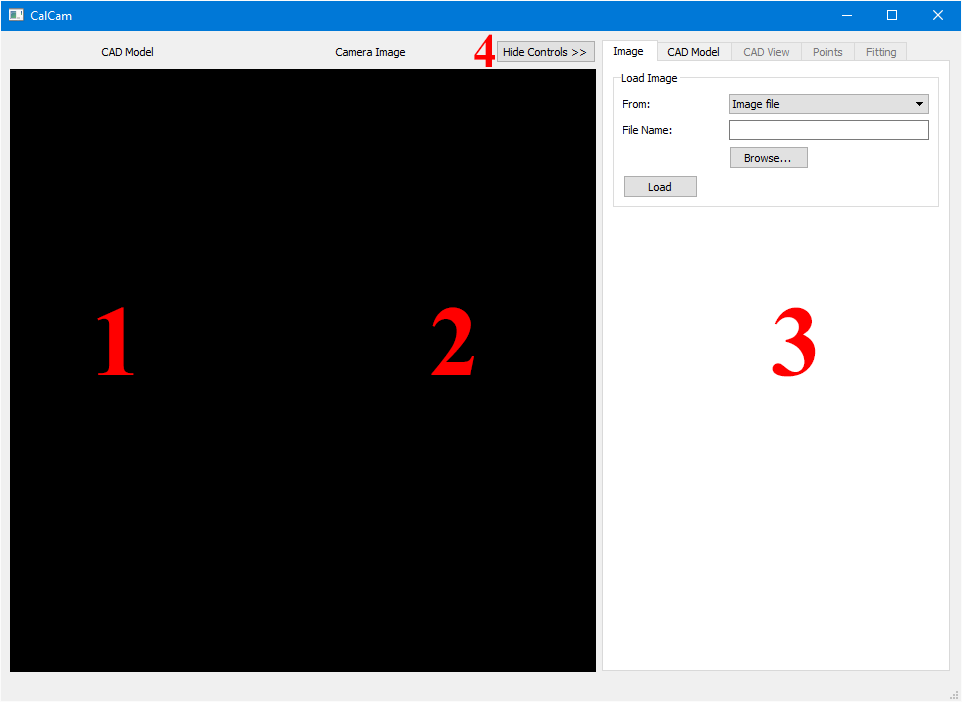
\includegraphics[width=\textwidth]{main_window.PNG}
\caption{\label{fig:main_window}Calcam main window.}
\end{figure}

You should be greeted with a window which looks like figure \ref{fig:main_window}. The main features of this window are, with reference to the numbers on the figure:

\begin{enumerate}
\item{\textbf{CAD Display:} the left half of the initially black area will be used to display the CAD model.}
\item{\textbf{Image Dipslay:} the right half of the initially black area will be used to display the camera image you are calibrating.}
\item{\textbf{Control tabs:} At the right-hand side of the window are a set of tabs which provide the controls for the program. These will be delt with in detail in the next sections. When the GUI is first loaded, only the Image and CAD model tabs will be enabled.}
\item{\textbf{Show / hide controls button:} Particularly on smaller screens, it is sometimes desirable to hide the control tabs to have a larger view of the image and CAD model while working. This button hides the control tabs, leaving the full window area for the CAD and image views. Clicking this button again re-opens the control tabs.}
\end{enumerate}

The following sections provide details on each step of performing a calibration.

\subsection{Loading and adjusting camera images}

The first step in performing a calibration is to load the camera image you wish to calibrate in to Calcam. The `Image' tab which is used to do this is open by default when the Calcam GUI starts. This tab is used to load an image or adjust the currently loaded image, and is shown in figure \ref{fig:im_tab}.

\begin{figure}[ht]
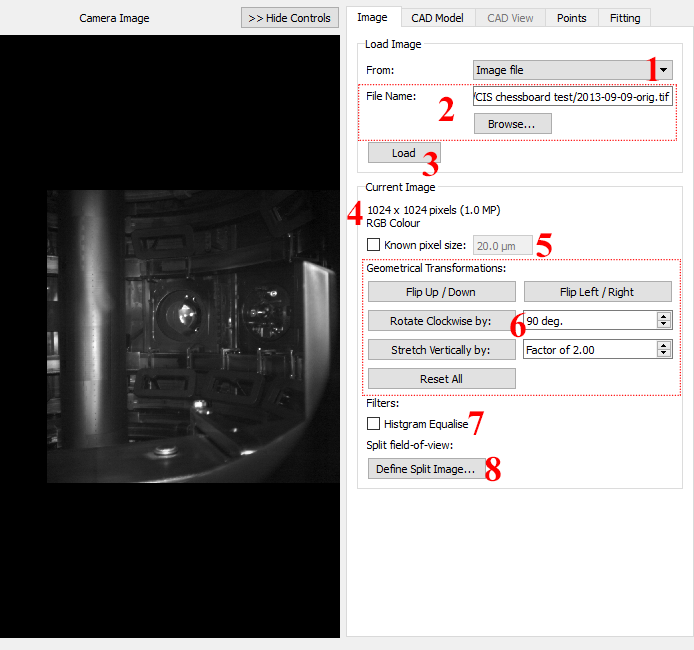
\includegraphics[width=\textwidth]{load_image.PNG}
\caption{\label{fig:im_tab} The image Tab.}
\end{figure}

\subsubsection{Loading Images}
At the top of the `Image' tab is a group of controls for loading images in to Calcam. This contains controls for loading an image:
\begin{enumerate}
\item{\textbf{``From'' dropdown box}\\Selects where the image should be loaded from (what image source should be used). The default is `Image File' which allows an image to be loaded from a normal image file. The other built-in option available is `Previously Used Image' which allows quick loading of an image used before in Calcam. If you have any user defined image sources (as described in section \ref{sec:image_sources}) they will also appear as an option here. }
\item{\textbf{Image Load Options}\\The controls here set the options for loading an image, and the displayed controls depend on the image source selected. In the case of loading an image file, a file name box appears which can be filled in manually or populated using the `Browse...' button to select a file.}
\item{\textbf{Load Button}\\Loads the image according to the options set above. The loaded image is displayed in the image view as shown in figure \ref{fig:im_tab}. Once the image is loaded, the `Current Image' section appears, and the Points and Fitting tabs are enabled.}
\end{enumerate}

Remember, as explained in section \ref{sec:im_coords}, it is highly recommended not to perform any rotation, flipping etc of the raw image before loading it, but instead to do these actions within calcam, as explained in the next section.

\subsubsection{Adjusting Images}

With an image loaded, the Image control tab contains a `Current Image' control group containing information and settings for the current image. If the image from the camera is not already the `right way up', this can be corrected here. If the camera system has multiple fields-of-view on the same detector, this can also be defined in this section. The controls in the `Current Image' section are:

\begin{enumerate}[resume]
\item{\textbf{Image Information}\\The pixel resolution and colour type are displayed at the top of the current image section. If the image dimensions are different in display and original coordinates (see section \ref{sec:im_coords}), both are displayed.}
\item{\textbf{Pixel Size}\\If the pixel size of the detector is known, it can be entered here. This is optional and does not effect the calibration except that calibrated focal lengths can be displayed in real length units rather than pixels. This is useful if you know what the effective focal length of the optical system should be, and want to sanity check the calibration.}
\item{\textbf{Geometrical Transformation Buttons}\\These buttons provide controls for rotating, flipping etc the image. If using these controls when some calibration points have already been defined, the calibration points are transformed with the image.}
\item{\textbf{Histogram Equalisation}\\This checkbox activates local histogram equalisation. This increases the contrast of features in the image, making them easier to identify and can therefore make it easier to accurately identify calibration points.}
\item{\textbf{Split field-of-view}\\Some camera diagnostics may have a split field-of-view, i.e. multiple, different views of the machine on the same detector, for example in optical systems using beam splitters or mirror boxes in the optical path. In this case, each sub field-of-view is calibrated independently. In order to do this, you must tell calcam which image pixels belong to which view. The `Define Split Image' button opens a dialog where you can define the split field-of-view. Full documentation for this dialog will be added later.}
\end{enumerate}

\subsection{Loading and working with CAD models}
Once the image to be calibrated has been loaded, the next step is to load the CAD model against which to calibrate the image. Calcam has two tabs concerned with the CAD model, described in the following sections.

\subsubsection{CAD Model Tab}

\begin{figure}[htb]
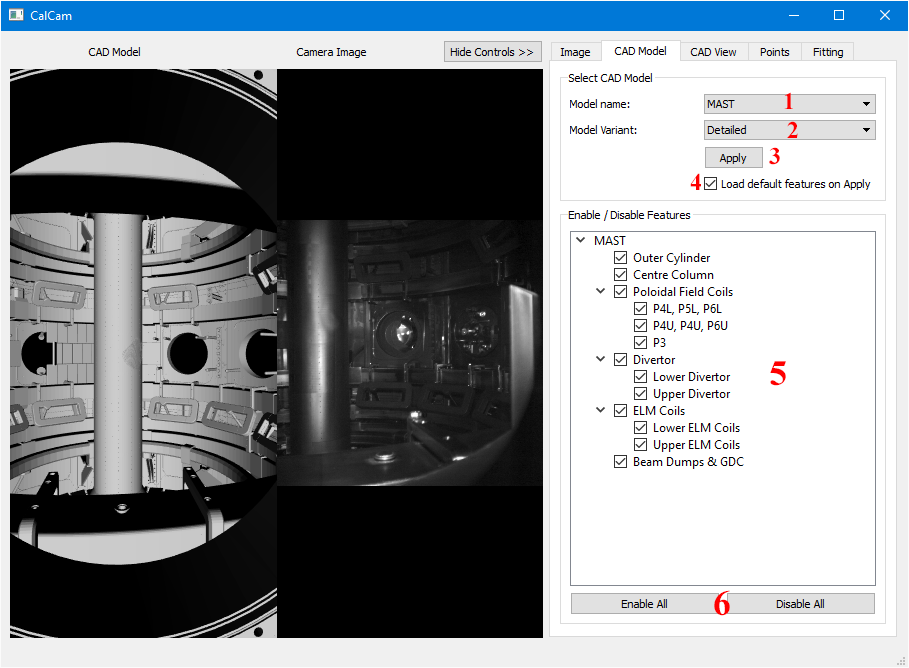
\includegraphics[width=\textwidth]{cad_model_tab.PNG}
\caption{\label{fig:cad_tab}CAD Model Tab.}
\end{figure}

The CAD Model tab is used to load or change CAD models, and turn on or off individual CAD model features in the view. This is shown in figure \ref{fig:cad_tab}. The controls on this tab are:

\begin{enumerate}
\item{\textbf{``Model Name'' dropdown box}\\This is used to select the CAD model to load, and lists all the CAD models which are configured (section \ref{sec:cad_config} describes how to configure CAD models). When a model is selected, the ``Model Variant'' dropdown box is populated with the available variants of the model, and set to the default variant specified in the CAD model definition.}
\item{\textbf{``Model Variant'' dropdown box}\\This is used to select a particular CAD model variant (as defined in the model configureation).}
\item{\textbf{Apply Button}\\ Loads the selected CAD model.} 
\item{\textbf{``Load default features on Apply'' Checkbox}\\ Controls what happens when the Apply button is clicked. If checked, which is the default, the Apply button will load all of the default features of the selected CAD model in to the CAD view. This can be undesirable for performance reasons if running on low specification systems when using large CAD models. If this box is unchecked, clicking Apply will populate the ``Enable / Disable Features'' box without loading the CAD data itself, allowing the user to load only the parts of the model they require.} 
\item{\textbf{Feature Selection}\\When a CAD model is loaded, this box ontains a checkable tree of all the individual ``features'' in the model. Checking or un-checking a feature, or group of features, will turn it on or off in the CAD view. This is useful to improve performance if not all parts of the CAD model are required, or if otherwise it is convenient to change which parts of the model are loaded.}
\item{\textbf{Enable / Disable All buttons}\\ These buttons enable or disable all the CAD model features in the above features list simultaneuosly.}
\end{enumerate}

\subsubsection{CAD View Tab}
\begin{figure}[htb]
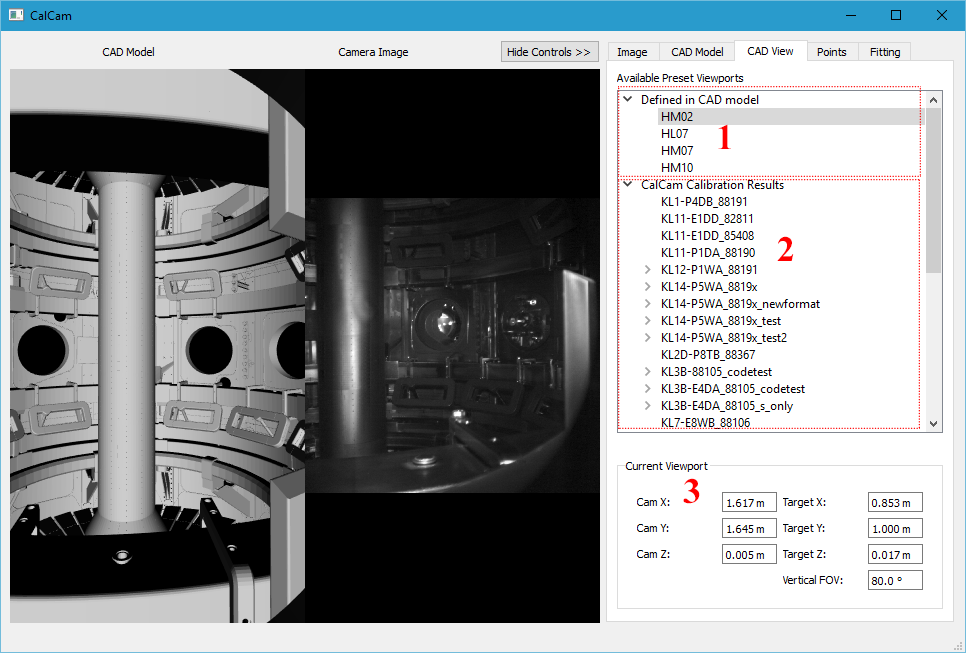
\includegraphics[width=\textwidth]{cad_view_tab.PNG}
\caption{\label{fig:cad_view_tab}The CAD View tab.}
\end{figure}
The CAD View tab is enabled when there is a CAD model loaded, and can be used to control or see information about the current CAD viewport. The view can be changed either interactively with the mouse (as described in the next section) and/or using the controls on this tab. The CAD View tab is shown in figure \ref{fig:cad_view_tab}, and has the following elements:

\begin{enumerate}
\item{\textbf{CAD Defined Viewports}\\This section lists all of the views configured in the CAD model definition. Clicking the name of a view sets the current CAD view to the clicked one.}
\item{\textbf{Calibration Results}\\This lists existing calcam calibration results. Clicking the name of a result will set the current CAD view to match the results of that calibration.}
\item{\textbf{Viewport Data}\\This section contains boxes showing the current CAD camera position coordinates, viewing target coordinates (the point towards which the camera is lookling), and CAD vertical field of view. These can be edited manually to change the CAD view or are updated to show the current values when the view is changed by another means.}
\end{enumerate}

\subsection{Defining points for calibration fitting}
\label{sec:editing_pointpairs}
With a CAD model and image loaded, you can begin to define calibration points by identifying matching features in the CAD model and camera image. In order to easily navigate around the image and CAD model to precisely place points, both the CAD and image views can be navigated with mouse controls.

\subsubsection{CAD View Mouse Controls}
The following controls can be used to navigate around the CAD model, with the mouse over the CAD view:

\begin{itemize}
\item{\textbf{Right Click + Drag}\\Look around (as in typical first person game controls)}
\item{\textbf{Middle Click + Drag}\\Pan (translate) the camera sideways}
\item{\textbf{Scroll Wheel up / down}\\ Move the camera forwards or backwards}
\item{\textbf{Ctrl + Scroll Wheel up / down}\\ Reduce / increase the camera field of view}
\end{itemize}

\subsubsection{Image View Mouse Controls}
The following controls can be used to navigate around the image view, with the mouse over the image:
\begin{itemize}
\item{\textbf{Middle Click + Drag}\\Pan around the image}
\item{\textbf{Scroll in / out}\\ Zoom in / out of current mouse pointer location}
\end{itemize}


\subsubsection{Adding or modifying Point Pairs}
Calcam uses `point pairs' to perform the calibration, where a point pair consists of one point on the CAD model and its corresponding point on the image. Point pairs are displayed on the CAD and image views as red {\color{red} +} cursors at the point locations. At any given time, one pair of points can be selected for editing. The selected point pair will be indicated with larger green {\color{green} +} cursors.

Once you have identified a common feature on the image and CAD model, \code{Ctrl + Click}  on the location on either the image or CAD view to create a new point pair. A point will be placed at the mouse location. Then click (without holding \code{Ctrl}) the corresponding point on the other view to finish creating the point pair. You should now see green {\color{green} +} cursors on both the CAD model and image. Clicking either the CAD model or image again will move the green cursor representing the current point to the clicked location. To start another point pair, \code{Ctrl + Click} again and repeat the process. The cursors showing the existing points will turn red, indicating they are no longer selected. In general, left clicking on either the image or CAD model will move the currently selected point to the clicked location. Clicking an existing cursor will select that point pair for editing, and holding \code{Ctrl} while clicking will start a new point pair.

If you start a new point pair but do not specify both CAD and image points (e.g. by \code{Ctrl+Click}ing on the image twice in a row), this will create `un-paired' points which will be ignored when setting up the fit. The cursors of these points will be displayed in yellow. You can go back to these later to add their corresponding point by clicking on the yellow cursor to select it, then clicking on the corresponding point in the other view. 

The currently selected point pair can be deleted by pressing the \code{Del} key on the keyboard, or clicking the ``Remove current point pair'' button on the Points control tab.

\subsubsection{Points Control Tab}

\begin{figure}[ht]
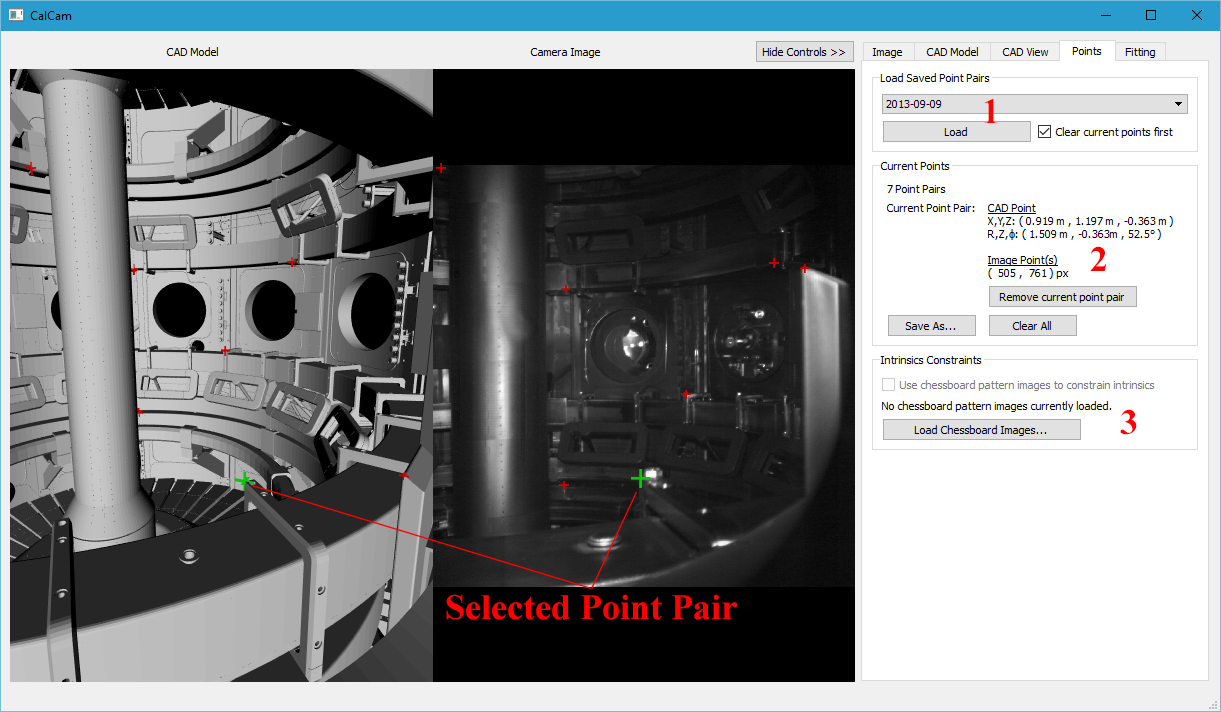
\includegraphics[width=\textwidth]{points_tab.PNG}
\caption{\label{fig:points_tab}The Points tab.}
\end{figure}
The points control tab contains 3 groups of controls used for loading, saving, inspecting and editing the calibration points, and is shown in figure \ref{fig:points_tab}. The controls are:

\begin{enumerate}
\item{\textbf{Load Saved Point Pairs}\\This allows loading of previously saved point pairs. The dropdown box contains a list of previously saved point pairs which can be loaded for use with the current image. By default, any existing point pairs are removed when the `Load' button is clicked, however un-checking the `Clear current pairs first' option will cause the loaded points to be added to any existing ones instead.}
\item{\textbf{Current Points}\\This section contains information and options about the currently defined point pairs. At the top of this section, the number of point pairs currently defined is shown (and the number of un-paired points, if there are any). Just below this is information about the currently selected point pair, which usually displays the CAD and image coordinates of the points (The information displayed about the CAD point location can be customised by defining a custom \code{get\_position\_info} method for your CAD model definitions, see section \ref{sec:cad_config}). The ``Remove current point pair'' button removes the currently selected point pair, while the ``Clear All'' button deletes all existing point pairs. The ``Save As...'' button allows the current point pairs to be saved for later use.}
\item{\textbf{Intrinsics Constraints}\\In many examples of real images, only a relatively small number of point pairs can be accurately identified. Due to the large number of free parameters in the camera model fit (focal length(s), centre of perspective and distortion parameters) this can give poor quality results. It is possible to better constrain the fits by using images of a chessboard pattern, with known square size, taken with the same camera + optical system configuration. This adds aditional constraints on the intrinsic model parameters, meaning only enough points to reliably fit the extrinsic parameters need to be identified in the image of the machine. Clicking the ``Load Chessboard Images...'' button opens a dialog box where you can load chessboard images to use as additional constraints. Once chessboard images have been loaded, they can be included or excluded from the fitting using the checkbox in this section. This user guide will later include guidelines on preparing chessboard images; for the time being, suitable advice can be found by searching for OpenCV camera calibration with chessboard images or the MATLAB camera calibration toolbox.}
\end{enumerate}

\subsection{Performing, checking and saving fits}

Once you have defined a set of point pairs, fitting is performed with the controls in the Fitting tab, shown in figure \ref{fig:fitting}. Before performing a fit, this tab contains only the `Fit Options' section, with the `Fit Results' section appearing once a fit has been performed.

\begin{figure}[ht]
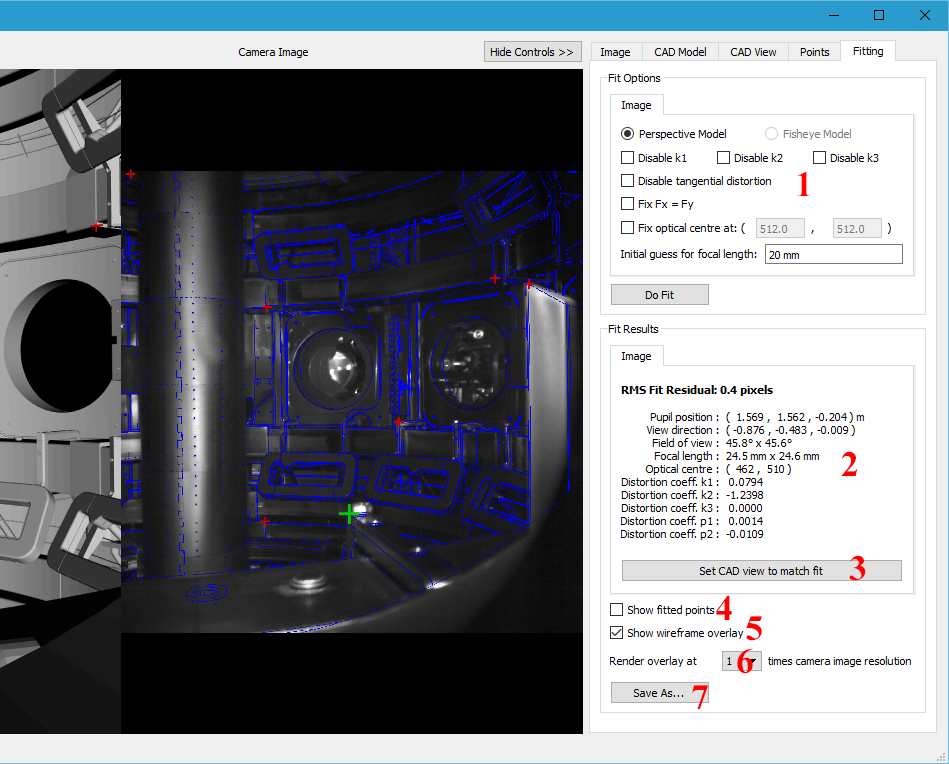
\includegraphics[width=\textwidth]{fitting.PNG}
\caption{\label{fig:fitting} The fitting control tab.}
\end{figure}

\subsubsection{Setting Fit Options and performing fits}
Fit options are adjusted using the top section on the Fitting control tab, marked (1) in figure \ref{fig:fitting}. The default options will typically produce good results for most images, however in some cases they will need to be adjusted to get a good quality result. For images with split fields of view, since each sub-field is fitted separately, tabs are displayed containing independent controls for each sub-field's fit options.

The first option to choose is whether to use the perspective or fisheye projection model: these two can be switched using the radio buttons at the top of the fit options section. The detailed options presented then depend on which model is selected:

\paragraph{Perspective Model Fit Options}

\begin{itemize}
\item{\textbf{Disable $k_1$...$k_3$}\\These options, when checked, set the corresponding coefficients in equation (\ref{eqn:perspective_distortion}) to be fixed at 0 in the fit. This changes the order of the radial distortion model (and disables radial distortion entirely if all three are checked). Disabling higher order radial distortion terms can improve fits when the point pairs do not sufficiently constrain the distortion model, when the fitted results can have large erroneous distortions.}
\item{\textbf{Disable Tangential Distortion}\\This option sets the coefficients $p_1$ and $p_2$ in equation (\ref{eqn:perspective_distortion}) to be fixed at 0 in the fit, i.e. disables tangential distortion in the fitted model. This can be helpful if the fitting results in large erroneous values of these coefficients.}
\item{\textbf{Fix $f_x = f_y$}\\This option fixes the focal lengths in the horizontal and vertical directions to be equal, i.e. fixes the image aspect ratio to 1. This is enabled by default, since for square pixels and non-anamorphic optics, which is the typical case, $f_x = f_y$ is expected. Un-checking this option can sometime help fit quality for some optical systems.}
\item{\textbf{Fix Optical Centre}\\This option fixes the location of the centre of perspective at the specified pixel coordinates. I'm not sure why you would ever want to use this, but since it's possible in the underlying OpenCV fitting, I thought I'd include the option.}
\item{\textbf{Initial Guess for Focal Length}\\This is the initial guess for the focal length used when starting the fit. The OpenCV fitter seems quite robust to values far from the final result, and the default value has been chosen to work well for most test images. However, there may be some cases where it is desirable to manually set the initial guess for the focal length for the fitter to find the correct solution.}
\end{itemize}


\paragraph{Fisheye Model Fit Options}
Note: fisheye model fits are only available if you are using OpenCV 3.
\begin{itemize}
\item{\textbf{Disable $k_1$...$k_4$}\\These options, when checked, set the corresponding coefficients in equation (\ref{eqn:fisheye_distortion}) to be fixed at 0 in the fit, changing the order of the fisheye distortion model.}
\item{\textbf{Initial Guess for Focal Length}\\This is the initial guess for the focal length used for the fitting. The OpenCV fitter seems quite robust to values far from the final result, and the default value has been chosen to work well for most test images. However, there may be some cases where it is desirable to manually set the initial guess for the focal length.}
\end{itemize}

To perform a fit using the current fit options, click the ``Do Fit'' button underneath the fit options. Alternatively, the keyboard shortcut \code{Ctrl+F} also performs a fit with the current settings.

\subsubsection{Checking fit quality and saving fits}
As soon as a fit is performed, the fitted points are shown on the image as blue {\color{blue} +} cursors. These are the current CAD model points, converted to image coordinates using the fitted model, i.e. for a good fit these should lie on top of the current image points. The fitted points can be turned on or off using the ``Show Fitted Points'' checkbox (4), or pressing \code{Ctrl+P} on the keyboard. The RMS fit error and fitted extrinsic and intrinsic parameters (camera pupil position and view direction, field of view, focal length, centre of perspective and distortion parameters) are dislayed in section (2). As with fit options, if the image has a split field-of-view, results for each field of view are shown on separate tabs. Note: for fits with small numbers of points, the camera model has sufficiently many free parameters that a very small RMS fit error can be obtained with a fit which is actually very bad! 

A more robust visual check of the fit quality can be obtained by overlaying the CAD model in wireframe on top of the camera image, according to the fit results. This is be done by checking the ``show wireframe overlay'' box (5) or pressing \code{Ctrl+O} on the keyboard. The CAD model is then rendered in wireframe and superimposed on the image. For large images or CAD models this can be very slow and memory intensive, and to improve the rendering speed or avoid memory errors, the resolution of the overlay can be reduced using the dropdown box (6). Conversely, the resolution of the overlay can be increased to allow more detail to be seen. It is also possible to set the current CAD viewport to approximate the fitted model using the `Set CAD view to match fit' button, which can be useful both for checking the fit and helping to identify point pairs.

Once a satisfactory fit has been obtained, the results can be saved using the `Save As...' button (7) at the bottom of the panel. This will also save the point pairs used for the fit, if this has not been done already. Once a satisfactory fit has been saved, this completes the calibration process using the calcam GUI.

\section{Using Calibrations: API Reference}
Once you have performed one or more calibration fits and saved the results, the Calcam Python API provides tools to make use of the results. The following sections document the most important modules and classes in Calcam for doing this.



\subsection{The \code{calcam.CalibResults} Class}
The class \code{calcam.CalibResults(fit\_name)} is used to represent calibration results, and has a number of methods for extracting useful information from the fitted model. To create a \code{CalibResults} instance representing a result saved with the name ``\code{foo}'' (this is the name used in the `Save As...' box when saving the result), initialise a \code{CalibResults} instance with the name as an argument: \code{MyFit = calcam.CalibResults(``fit\_name'')}. This searches for a file \path{~/calcam/FitResults/fit_name.pickle}, which is where clacam stores its fit results, and loads the results stored in that file. A summary of the fit results, similar to that displayed in the Calcam GUI after fitting, can be seen by using the print statement on the resulting object, i.e. \code{print(MyFit)}. The main useful methods of the \code{CalibResults} class are:

\subsubsection*{\code{get\_pupilpos([x\_pixels,y\_pixels,field,Coords])}}
\begin{adjustwidth}{0.5cm}{0cm}
Get the camera pupil position, i.e. the origin of the camera's sight-lines, in the lab (i.e. CAD model) coordinate system. 
\subsubsection*{Inputs}
For the common case of an image without a split field of view, no arguments are necessary and this can be called as \code{get\_pupilpos()}. For images with a split field-of-view, optional input arguments are:
\begin{itemize}
\item{\code{x\_pixels={\it None}, y\_pixels={\it None}}\\ Array-likes of floats containing the X and Y pixel coordinates you want to know the pupil position for. This is only useful or necessary for optical systems with split fields-of-view, where not all pixels necesserily have the same pupil position. Eiether this or \code{field} must be specified for split field-of-view images.}
\item{\code{field=0}\\For split field-of-view cameras, an integer specifying the number of the sub-field you want the pupil position for.}
\item{\code{Coords=`Display'}\\String, either `Display' or `Original': if specifying x\_pixels and y\_pixels, this specifies whether the input x and y pixel coodinates are in display or original coordinates.}
\end{itemize}
\subsubsection*{Outputs} 
\begin{itemize}
\item{3-element array of floats containing the camera pupil position \code{(X,Y,Z)} in metres.}
\end{itemize}
\end{adjustwidth}

\subsubsection*{\code{get\_fov([field])}}
\begin{adjustwidth}{0.5cm}{0cm}
Get the horizontal and vertical field of view of the camera in degrees. 
\subsubsection*{Inputs}
For the common case of an image without a split field of view, no arguments are necessary and can be called as \code{get\_fov()}. For images with a split field-of-view, optional input arguments are:
\begin{itemize}
\item{\code{field=0}\\Index of the sub field-of-view for which to get the view angles.}
\end{itemize}
\subsubsection*{Outputs} 
\begin{itemize}
\item{Two element array containing the \code{(horiz,vert)} field-of-view in degrees.}
\end{itemize}
\end{adjustwidth}


\subsubsection*{\code{get\_los\_direction([x\_pixels,y\_pxels,Coords])}}
\begin{adjustwidth}{0.5cm}{0cm}
Get unit vectors representing the directions of the camera's sight-lines in the lab (CAD Model) coordinate system.
\subsubsection*{Inputs}
If called with no input arguments, this function returns the sight-line directions of every pixel in the image. Optional inputs are:
\begin{itemize}
\item{\code{x\_pixels={\it None},y\_pixels={\it None}}\\Pixel coordinates for which to return the lines of sight. If none are given, results are returned for all pixels in the image. \code{x\_pixels} and \code{y\_pixels} can be any shape, as long as they are the same shape as each other.}
\item{\code{Coords=`Display'}\\String, either `Display' or `Original': if specifying \code{x\_pixels} and \code{y\_pixels}, this specifies whether the input x and y pixel coodinates are in display or original coordinates. If \code{x\_pixels} and \code{y\_pixels} are not given, this controls whether the output corresponds to the image in display or original coordinates. }
\end{itemize}
\subsubsection*{Outputs} 
\begin{itemize}
\item{NumPy array containing 3D unit vectors whose directions are the sight-line directions in the lab frame. If no pixel coordinates are given this will be a $[h\: \mathrm{x} \: w \: \mathrm{x}\: 3]$ array, where $w$ and $h$ are the image width and height, and the third axis contains the (X,Y,Z) components of the sight-line unit vectors. If \code{x\_pixels} and \code{y\_pixels} are given, the output array will be the same shape as \code{x\_pixels} and \code{y\_pixels} with an additional axis added to store the 3 components of the sight-line vectors (i.e. if x\_pixels is a 5x5 array, the output will be 5x5x3). }
\end{itemize}
\end{adjustwidth}

\subsubsection*{\code{project\_points(ObjPoints,[CheckVisible,RayData,RayCaster,\\VisibilityMargin,Coords])}}
\begin{adjustwidth}{0.5cm}{0cm}
Project given 3D points in the lab frame in to pixel coordinates on the image. Optionally, checks whether the given points are visible in the image or occluded by geometry in the CAD model.
\subsubsection*{Inputs}
\begin{itemize}
\item{\code{ObjPoints}\\3D point coordinates to project on to the detector. These can be specified by EITHER an Nx3 array, where N is the number of points, or an array-like of 3 element arrays, where each 3 element array specifies a point.}
\item{\code{CheckVisible={\it False}}\\Bool, whether to check if the 3D points are visible to the camera or hidden behind CAD geometry. If this is set to \code{True}, either \code{RayData} or \code{RayCaster} must also be specified.}
\item{\code{RayData={\it None}}\\A \code{calcam.RayData} object containing sight-line information for this view, used for checking point visibility if this is requested. If both \code{RayData} and \code{RayCaster} are specified, this will not be used.}
\item{\code{RayCaster={\it None}}\\A \code{calcam.raytrace.RayCaster} object for this camera view and CAD model, used for checking point visibility if this is requested. If both \code{RayData} and \code{RayCaster} are specified, this will override \code{RayData}.}
\item{\code{VisibilityMargin=0}\\A fudge factor to adjust the behaviour of \code{CheckVisibility}, I can't remember why I introduced this. This is a distance in metres, such that points this far behind a CAD feature will still be considered visible to the camera.}
\item{\code{Coords=`Display'}\\String, either `Display' or `Original': whether the resulting image coordinates should be in original or display coordinates.}
\end{itemize}
\subsubsection*{Outputs} 
\begin{itemize}
\item{\code{ImagePoints}\\A list of Nx2 numpy arrays containing the image coordinates of the given 3D points. Each array contains the list of image pixel coordinates [x,y] for a sub-field of view of the image. For simple images without a split field of view, \code{ImagePoints} is a one-element list where \code{ImagePoints[0]} is an Nx2 array containing the image coordinates. Points not visible to the camera, either because their projection is off the image edge, or they are occluded and CheckVisible is enabled, will have their image coordinates set to \code{[np.nan,np.nan]}. }
\end{itemize}
\end{adjustwidth}

\subsubsection*{\code{get\_cam\_to\_lab\_rotation([field])}}
\begin{adjustwidth}{0.5cm}{0cm}
Get a 3D rotation matrix which rotates from the camera frame to the lab frame. This is mostly used internally in calcam, but might be useful.
\subsubsection*{Inputs}
For the common case of an image without a split field of view, no arguments are necessary and can be called as \code{get\_cam\_to\_lab\_rotation()}. For images with a split field-of-view, optional input arguments are:
\begin{itemize}
\item{\code{field=0}\\Index of the sub field-of-view for which to get the view angles.}
\end{itemize}
\subsubsection*{Outputs} 
\begin{itemize}
\item{3x3 NumPy matrix containing the rotation matrix.}
\end{itemize}
\end{adjustwidth}

\subsection{The \code{CADModel} Class}
The functions described in the following sections require Calcam CAD model objects as inputs, therefore the CAD model class is very briefly documented here. This is the parent class for user-defined CAD models in calcam, and provides methods both for user interaction and interaction with the rest of calcam. 

To create a CAD model instance representing a given model, use \code{model = calcam.machine\_geometry.model\_name([`model\_variant'])}, where \code{model\_name} is the name of the user-defined CAD model class and `model\_variant' is an optional string specifying the model variant (the default used when model\_variant is not specified is configured in the CAD model definition). For more details about how these names are configured, see the example CAD model definition example/template as described in section \ref{sec:cad_config}.

The most useful methods of the CAD model class for the user are:
\subsubsection*{\code{enable\_features(feature\_list)}}
\begin{adjustwidth}{0.5cm}{0cm}
Enable the given features of the model. When a new CAD model instance is initialised, features will automatically be enabled according to the configuration in the CAD model definition. Enabling features means their CAD data will be loaded and they will be included in rendering, ray casting etc.
\subsubsection*{Inputs}
\begin{itemize}
\item{\code{features}\\A list of strings with the names of the features to be enabled.}
\end{itemize}
\end{adjustwidth}
\subsubsection*{\code{disable\_features(feature\_list)}}
\begin{adjustwidth}{0.5cm}{0cm}
Disable the given features of the model. When a new CAD model instance is initialised, features will automatically be enabled according to the configuration in the CAD model definition. Disabling features means their CAD data will not be loaded and they will be excluded from rendering, ray casting etc.
\subsubsection*{Inputs}
\begin{itemize}
\item{\code{features}\\A list of strings with the names of the features to be disabled.}
\end{itemize}
\end{adjustwidth}
\subsubsection*{\code{enable\_only(feature\_list)}}
\begin{adjustwidth}{0.5cm}{0cm}
Enable only the given features of the model, disabling all others.
\subsubsection*{Inputs}
\begin{itemize}
\item{\code{features}\\A list of strings with the names of the features to be enabled.}
\end{itemize}
\end{adjustwidth}
\subsubsection*{\code{set\_colour(Colour,[feature\_list])}}
\begin{adjustwidth}{0.5cm}{0cm}
Set the colour in which the CAD model should appear, either for the whole model or particular features.
\subsubsection*{Inputs}
\begin{itemize}
\item{\code{Colour}\\A 3-element list or tuple of values between 0 and 1 giving the (R,G,B) desired colour.}
\item{\code{Features={\it None}} A list of strings containing the feature names to which this colour should be applied. If none, the colour is applied to the whole model.}
\end{itemize}
\end{adjustwidth}
\subsubsection*{\code{enable\_only(feature\_list)}}
\begin{adjustwidth}{0.5cm}{0cm}
Enable only the given features of the model, disabling all others.
\subsubsection*{Inputs}
\begin{itemize}
\item{\code{features}\\A list of strings with the names of the features to be enabled.}
\end{itemize}
\end{adjustwidth}
\subsubsection*{\code{get\_enabled\_features()}}
\begin{adjustwidth}{0.5cm}{0cm}
Get a list of the currently enabled features.
\subsubsection*{Output}
\begin{itemize}
\item{\code{features}\\List of strings of the names of enabled features.}
\end{itemize}
\end{adjustwidth}
\subsubsection*{\code{colour\_by\_material(on)}}
\begin{adjustwidth}{0.5cm}{0cm}
Set whether the CAD model features should be coloured according to their different physical materials.
\subsubsection*{Inputs}
\begin{itemize}
\item{\code{on}\\Bool, whether or not to turn on colouring according to material. The default is set in the CAD model definition.}
\end{itemize}
\end{adjustwidth}
\subsubsection*{\code{flat\_shading(on)}}
\begin{adjustwidth}{0.5cm}{0cm}
Turn on or off flat shading. When enabled, this disabled all lighting effects when the CAD model is rendered, showing it as flat colours.
\subsubsection*{Inputs}
\begin{itemize}
\item{\code{on}\\Bool, whether or not to turn on flat shading.}
\end{itemize}
\end{adjustwidth}
\subsubsection*{\code{colour\_by\_material(on)}}
\begin{adjustwidth}{0.5cm}{0cm}
Set whether the CAD model features should be coloured according to their different physical materials.
\subsubsection*{Inputs}
\begin{itemize}
\item{\code{on}\\Bool, whether or not to turn on colouring according to material. The default is set in the CAD model definition.}
\end{itemize}
\end{adjustwidth}

\subsection{The Render Module}
The module \code{calcam.render} contains functions related to rendering images from calibration results. It contains one main important function:
\subsubsection*{\code{render\_cam\_view(CADModel,FitResults[,...])}}
\begin{adjustwidth}{0.5cm}{0cm}
Render the given CAD model, from the point of view of a camera described by the calibration results object \code{FitResults}. This renders the CAD model including the correct image distortion.
\subsubsection*{Inputs}
\begin{itemize}
\item{\code{CADModel}\\A calcam CAD model object containing the CAD model to render.}
\item{\code{FitResults}\\A \code{calcam.CalibResults} object containing the fit results to base the rendering upon.}
\item{\code{filename={\it None}}\\String, an image file name to save the resulting rendered image (including file extension).}
\item{\code{oversampling=1}\\The rendered image size in pixels will be equal to this number multiplied by the actual camera resolution. Must be $2^N$ where $N$ is an integer (including negative integers, if rendering at a smaller resolution than the original camera is desired).}
\item{\code{AA=1}\\Factor by which to oversize the intermediate render, for antialiasing. Largeer values reduce blocky edges in the resulting images but quickly become very memory intensive to render.}
\item{\code{Edges=False}\\Bool, if set to \code{True}, the CAD model is rendered in wireframe, otherwise it is rendered as solid.}
\item{\code{EdgeColor=(1,0,0)}\\If rendering in wireframe, a tuple of 3 values from 0-1 specifying the RGB colour of the wireframe.}
\item{\code{EdgeWidth}\\If rendering in wireframe, the thickness in pixels of the wireframe lines.}
\item{\code{Transparendcy=False}\\Bool, whether to make the background transparent. If left at the default \code{False}, the background will be black.}
\item{\code{EdgesMethod=None}\\A string, if rendering in wireframe, this can be used to override the CAD model's default edge type used for the wireframe. \\code{EdgeMethod=Simple} shows all polygon edges of the CAD model, while \code{EdgeMethod=Detect} more intelligently detects edges.}
\item{\code{Coords=`Display'}\\Whether to render in original or display image orientation.}
\end{itemize}
\subsubsection*{Outputs}
\begin{itemize}
\item{NumPy array containing the rendered image: a $[h\:\mathrm{x}\:w\:\mathrm{x}\:3]$ or $[h\:\mathrm{x}\:w\:\mathrm{x}\:4]$ (if using transparency) array containing the rendered RGB or RGBA image.}
\item{If a filename is given, the function also saves the rendered image to a file with the given name (note: if transparency is enabled, any given file type will be overriden to PNG).}
\end{itemize}
\end{adjustwidth}

\subsection{The RayCaster Class}
The class \code{calcam.raytrace.RayCaster([FitResults,CADModel])} is used for ray casting, i.e. to find the points of intersection between the camera sight lines and machine structure. It can be initialised with or without specifying the calibration results and CAD model to use.

\subsubsection*{\code{set\_cadmodel(CADModel)}}
\begin{adjustwidth}{0.5cm}{0cm}
Sets the CAD model to be used for the raycasting: takes a calcam CAD model instance as input.
\end{adjustwidth}

\subsubsection*{\code{set\_calibration(CalibResults)}}
\begin{adjustwidth}{0.5cm}{0cm}
Sets the calibration fit results used for the raycasting: takes a CalibResults instance as input.
\end{adjustwidth}

\subsubsection*{\code{raycast\_pixels([x,y,binning,Coords])}}
\begin{adjustwidth}{0.5cm}{0cm}
Perform raycast to find points of intersection between pixel sight-lines and CAD geometry.
\subsubsection*{Inputs}
\begin{itemize}
\item{\code{x,y}\\x and y pixel coordinates for which to perform the ray casting. If none are specified, the function will ray cast each pixel on the detector. Can be any size or shape, as long as the size of x and y are the same.}
\item{\code{binning=1}\\If ray casting the entire detector without specifying any pixel coordinates, controls the binning of the detector for raycasting. If binning is set to N, the ray cast is performed with the detector binned by a factor NxN.}
\item{\code{Coords=`Display'}\\ If x and y are given, specifies whether the given coordinates are in display or original coordinates. If no x and y are given, determines whether the raycast is performed in original or display coordinates.}
\end{itemize}

\subsubsection*{Outputs}
\begin{itemize}
\item{RayData - a calcam RayData object containing the raycast results.}
\end{itemize}
\end{adjustwidth}

\subsection{The RayData Class}
The \code{RayData(raydata\_name)} class is used to store the results from raycasting. Existing results are loaded by initialising with the name of some saved RayData. This is the type of object returned by the \code{calcam.raytrace.RayCaster.raycast\_pixels}.

\subsubsection{Properties}

\subsubsection*{\code{ray\_end\_coords}}
\begin{adjustwidth}{0.5cm}{0cm}
Numpy array containing the sight-line end points, i.e. the coordinates where the sight-lines intersect the CAD model. The shape of the array is the same as the shape of the input coordinates for the raycast, plus one extra dimension. The final dimension of the array will have length 3 and represent the X, Y and Z coordinates of the ray end point in metres.
\end{adjustwidth}

\subsubsection*{\code{ray\_start\_coords}}
\begin{adjustwidth}{0.5cm}{0cm}
Array containing the origin of the sight-lines, i.e. the camera pupil position. This will be the same as the result from \code{CalibResults.get\_pupilpos}.  The shape of the array is the same as the shape of the input coordinates for the raycast, plus one extra dimension. The final dimension of the array will have length 3 and represent the X, Y and Z coordinates of the ray start point in metres.

\end{adjustwidth}

\subsubsection*{\code{x} and \code{y}}
\begin{adjustwidth}{0.5cm}{0cm}
Arrays containing the x and y pixel locations of each raycast pixel. These are the same shape as  the input coordinates for the raycast, and are always in display coordinates.
\end{adjustwidth}


\subsubsection{Methods}
\subsubsection*{\code{get\_ray\_lengths([x,y,PositionTol,Coords])}}
\begin{adjustwidth}{0.5cm}{0cm}
Returs the length of the sight-lines for the specified pixel coordinates, i.e. the distance from the camera pupil where the sight lines intersect the CAD geometry.
\subsubsection*{Inputs}
\begin{itemize}
\item{\code{x} and \code{y}\\x and y pixel coordinates at which to return the sight line length. Must be the same size as each other. If none are specified, returns the result for every pixel in the raycast result.}
\item{PositionTol=3\\It is possible that the raycast was not performed at exactly the specified pixel x and y coordinates. Normally, this function will return the result from the closest point which was raycast, provided the distance of that point is within \code{PositionTol} pixels of the requested coordinates.}
\item{\code{Coords=`Display'}\\ If x and y are given, specifies whether the given coordinates are in display or original coordinates. If no x and y are given, determines whether the output should be returned in original or display coordinates.}
\end{itemize}
\subsubsection*{Outputs}
\begin{itemize}
\item{Numpy array containing the sight-line lengths in metres. If x and y are specified, this is the same shape as x and y. If no x and y are specified, this is the same shape as the x and y inputs to the raycast.}
\end{itemize}
\end{adjustwidth}

\subsubsection*{\code{get\_ray\_directions([x,y,PositionTol,Coords])}}
\begin{adjustwidth}{0.5cm}{0cm}
Returns unit vectors representing the direction of the camera sight-lines in the lab frame. Does the same job as \code{CalibResults.get\_los\_direction} (maybe I should rename this one to match?).
\subsubsection*{Inputs}
\begin{itemize}
\item{x, y\\x and y pixel coordinates at which to return the sight line directions. Must be the same size as each other. If none are specified, returns the result for every pixel in the raycast result.}
\item{PositionTol=3\\It is possible that the raycast was not performed at exactly the specified pixel x and y coordinates. Normally, this function will return the result from the closest point which was raycast, provided the distance of that point is within PositionTolerance pixels of the requested coordinates.}
\item{\code{Coords=`Display'}\\ If x and y are given, specifies whether the given coordinates are in display or original coordinates. If no x and y are given, determines whether the output should be returned in original or display coordinates.}
\end{itemize}
\end{adjustwidth}
\subsubsection*{Outputs}
\begin{itemize}
\item{Numpy array containing 3D unit vectors representing the sight-line directions in the lab frame.}
\end{itemize}
\subsection{The Geometry Matrix Module}
The geometry matrix module is used to produce geometry matrices for tomographic reconstruction of plasma emissivity profiles, assuming toroidal symmetry. There is currently no documentation for this module in this document; the module RO is James Harrison.
\end{document}

